\documentclass{scribe-cgenomics}
\usepackage{float}
\usepackage{subfig}
\usetikzlibrary{matrix, positioning}
\usepackage{mathtools}
\usepackage{tkz-euclide}

\begin{document}

\جلسه
{دکتر کسری علیشاهی، ترم دوم سال تحصیلی ۱۴۰۰}
{تمرین نظری}
{محسن قدرتی}


% ------------------------------------------------------
% problem 1
% ------------------------------------------------------
\newpage
\begin{prob}

\end{prob}

\begin{حل}
 احتمال پیشامد
$n$
بار شیر آمدن در
$2n$
پرتاب یک سکه را
$\theta_n$
بنامیم. داریم:

\begin{center}
$
\theta_n =
\begin{pmatrix}
2n \\ n
\end{pmatrix}
\dfrac{1}{2^{2n}}
= \dfrac{(2n)!}{n!n!2^{2n}}
$
\end{center}

تقریب استرلینگ برای
$n!$
به صورت زیر است:

\begin{center}
$
n! \simeq \sqrt{2\pi n}(\dfrac{n}{e})^{n}
$
\end{center}

در نتیجه

\begin{center}
$
\theta_n \simeq 
\dfrac{\sqrt{2\pi 2n}(\dfrac{2n}{e})^{2n}}{\sqrt{2\pi n}(\dfrac{n}{e})^n \sqrt{2\pi n}(\dfrac{n}{e})^n 2^{2n}}
= \dfrac{1}{\sqrt{\pi n}} \dfrac{2^{2n}n^{2n}e^{-2n}}{2^{2n} n^n e^{-n}n^n e^{-n}}
= \dfrac{1}{\sqrt{\pi n}}
$
\end{center}

پس به ازای
$n=50$،

\begin{center}
$
\theta_{50} \simeq \dfrac{1}{\sqrt{50\pi}} \simeq 0.0797
$
\end{center}

به طور کلی از رابطه بالا نتیجه می‌شود
$\theta_n = 2\theta_{4n}$.
یعنی
$\theta_n$
در حال کاهش است از مرتبه رادیکالی است. که توجیه این موضوع افزایش تعداد حالات تقریبا معادل است. مثلا احتمال
$n-1$
بار شیر آمدن در
$2n$
پرتاب، با
$\theta_n$
در
$n$های
بزرگ تفاوت خاصی ندارد.

\end{حل}



% ------------------------------------------------------
% problem 2
% ------------------------------------------------------
\newpage
\begin{prob}

\end{prob}

\begin{حل}
فرض کنیم در حالت کلی‌تر،
$n$
مهره در ظرف قرار دارد و
$2n$
بار نمونه‌گیری با تکرار کرده‌ایم. اگر متغیر تصادفی
$X_i$
را برابر با تعداد دفعات مشاهده توپ
$i$ام
تعریف کنیم، به دنبال
$E[\delta_{X_1-1} + \delta_{X_2-1} + \dots + \delta_{X_n-1}]$
هستیم. داریم:

\begin{center}
$
E[\delta_{X_1-1} + \delta_{X_2-1} + \dots + \delta_{X_n-1}]
= E[\delta_{X_1-1}] + \dots + E[\delta_{X_n-1}]
$
\end{center}

اما
$X_i$ها
هم‌توزیع هستند و به ازای هر کدام داریم

\begin{center}
$
E[\delta_{X_i-1}] = Pr[X_i = 1]
= \dfrac{2n (n-1)^{2n-1}}{n^{2n}}
= 2(1-\dfrac{1}{n})^{2n-1}
\simeq 2\exp({-\dfrac{2n-1}{n}})
\simeq \dfrac{2}{e^2} 
\simeq 0.27067
$
\end{center}

که در آن، روش شمارش به این ترتیب است که ابتدا مهره
$i$ام
را جایی در دنباله قرار می‌دهیم و سپس بقیه خانه‌های دنباله را از بین بقیه مهره‌ها انتخاب می‌کنیم. پس

\begin{center}
$
E[\delta_{X_1-1} + \delta_{X_2-1} + \dots + \delta_{X_n-1}]
\simeq 2ne^{-2} 
\qquad \implies \qquad
E[\delta_{X_1-1} + \dots + \delta_{X_{100}-1}]
\simeq 27.067
$
\end{center}

\vspace*{1in}

احتمال آنکه همه مهره‌ها دیده شوند (با توجه به هم‌توزیع بودن و تقارن
$X_i$ها)
عبارت است از:

\begin{center}
$
Pr[X_1\geq 1,\ \dots,\ X_n\geq 1]
= 1 - Pr[X_1=0 \cup \dots \cup X_n=0]
$
\bigbreak
$= 1 - nPr[X_1=0]
+\begin{pmatrix}
n\\ 2
\end{pmatrix}
Pr[X_1=0,\ X_2=0] -\dots
$
\bigbreak
$
=
1 - 
\begin{pmatrix}
n\\1
\end{pmatrix}
\dfrac{(2n)^{n-1}}{(2n)^n}
+
\begin{pmatrix}
n\\2
\end{pmatrix}
\dfrac{(2n)^{n-2}}{(2n)^n}
- \dots +
(-1)^n \begin{pmatrix}
n\\n
\end{pmatrix}
\dfrac{(2n)^{n-n}}{(2n)^n}
$
\bigbreak
$
= \sum_{i=0}^{n}(-1)^i \begin{pmatrix}
n\\i
\end{pmatrix}
\dfrac{1}{(2n)^i}
= (1 - \dfrac{1}{2n})^n
\simeq \exp(-\dfrac{n}{2n}) 
= e^{-2} \simeq 0.135
$
\end{center}

پس یک تقریب از احتمال دیده شدن همه گوی‌ها برابر است با
$0.135$.

\end{حل}




% ------------------------------------------------------
% problem 3
% ------------------------------------------------------
\newpage
\begin{prob}
\end{prob}

\begin{حل}

هنگامی که چوب از یک نقطه تصادفی شکسته باشد، اگر طول قطعه بزرگتر را
$L$
بنامیم، خواهیم داشت:

\begin{center}
$
E(L) = 
\int_{0}^{0.5} 1-x dx + \int_{0.5}^{1} xdx
= (x-\dfrac{x^2}{2})\big]_{0}^{0.5} + (\dfrac{x^2}{2})\big]_{0.5}^{1}
= \dfrac{1}{2} - \dfrac{1}{8} + \dfrac{1}{2} - \dfrac{1}{8} 
= \dfrac{3}{4}
$
\end{center}

پس اگر نسبت میانگین طول قطعه بزرگ‌تر ($L$) به میانگین طول قطعه کوچک‌تر ($S$) را بخواهیم، از آنجا که در هر نمونه‌گیری
$L+S=1$
خواهیم داشت:

\begin{center}
$
\dfrac{E(L)}{E(S)} = \dfrac{\frac{3}{4}}{1 - \frac{3}{4}} = 3
\..
$
\end{center}

اما اگر به دنبال
$E(\dfrac{L}{S})$
هستیم، داریم:

\begin{center}
$
\int_{0}^{0.5} \dfrac{1-x}{x} dx + \int_{0.5}^{1} \dfrac{x}{1-x} dx
= \int_{0}^{0.5} \dfrac{1}{x} - 1 dx + \int_{0.5}^{1} \dfrac{1}{1-x} - 1 dx
= (\log x - x)\big]_{0}^{0.5} + (-\log (1-x)-x)\big]_{0.5}^{1}
$
\bigbreak
$
=( -\log 2 - \dfrac{1}{2} - \lim_{x\rightarrow 0^+}\log x)
+ (- \lim_{x\rightarrow 0^+}\log x - 1 -\log 2 + \dfrac{1}{2})
= \infty
$
\end{center}

دلیل اتفاق بالا آن است که مقادیر
$\dfrac{L}{S}$
می‌توانند بدون کران بزرگ باشند و بر اساس نتیجه بالا نیز مشخص است که مقادیر بسیار بزرگ چگالی غیرقابل چشم‌پوشی دارند.

\vspace*{1in}

هنگامی که چوب از دو نقطه تصادفی مستقل و با توزیع یکنواخت شکسته باشد، اگر طول سه قطعه بزرگتر، متوسط و کوچک‌تر را به ترتیب
$L$،
$M$
و
$S$
بنامیم، چون متغیرهای
$X_1$
و
$X_2$
مستقل از یکدیگرند، می‌توانیم فرض کنیم که به طور یکنواخت، از نقاط یک مربع یک در یک انتخاب شده‌اند. برای راحتی بیشتر در کار با متغیر‌ها نیز، فرض کنیم به جای
$X_1$
و
$X_2$
متغیرهای تصادفی مذکور را
$X$
و
$Y$
بنامیم.

\begin{figure}[h]
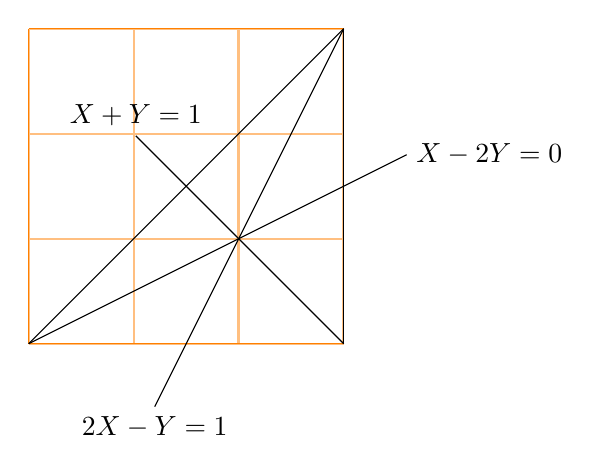
\begin{tikzpicture}[scale=4]
   \tkzInit[xmax=1,ymax=1,xmin=0,ymin=0]
   \tkzGrid[sub,color=orange,subxstep=.333,subystep=.333]
   \tkzAxeXY
   \draw[-] (0,0) -- (1.2,0.6) node[anchor=west] {$X-2Y=0$};   
   \draw[-] (1,0) -- (0.34,0.66) node[anchor=south] {$X+Y=1$};
   \draw[-] (1,1) -- (0.4,-0.2) node[anchor=north] {$2X-Y=1$};
   \draw[-] (1,1) -- (1,0);
   \draw[-] (0,0) -- (1,1);
  \end{tikzpicture}
  \centering
\end{figure}

مساله دارای تقارن است 
\cite{stick_countor}. 
به این ترتیب که احتمال هر یک از پیشامد‌های زیر برابر با مساحت یک چهارضلعیست که براحتی می‌توان مشاهده کرد برابر با
$\dfrac{1}{6}$
است.

\begin{center}
$
Pr(L=Y) = Pr(L=1-X) = Pr(L=X-Y) = \dots = \dfrac{1}{6}
$
\end{center}

از طرفی توجه می‌کنیم که هر پیشامد
$\{(X,Y)\ |\ X\geq Y,\ L=Y\}$
توسط تناظر‌های داده شده با هر پیشامد زیر متناظر است:

\begin{center}
$
\begin{cases}
(X',\ Y') := (1-Y,\ 1-X) & 
\qquad \{(X',Y')\ |\ X'\geq Y',\ L=1-X'\}\\
(X',\ Y') := (1-X+Y,\ 1-X) & 
\qquad \{(X',Y')\ |\ X'\geq Y',\ L=X'-Y'\}\\
(X',\ Y') := (Y,\ X) & 
\qquad \{(X',Y')\ |\ X'\leq Y',\ L=X'\}\\
(X',\ Y') := (1-X,\ 1-Y) & 
\qquad \{(X',Y')\ |\ X'\leq Y',\ L=1-Y'\}\\
(X',\ Y') := (X-Y,\ X) & 
\qquad \{(X',Y')\ |\ X'\geq Y',\ L=Y'-X'\}\\
\end{cases}
$
\end{center}

پس احتمال‌های شرطی زیر نیز برابرند:

\begin{center}
$
Pr(L\leq l\ |\ L=Y) = Pr(L\leq l\ |\ L=1-X) =Pr(L\leq l\ |\ L=X-Y) = \dots
$
\end{center}

پس طبق قانون احتمال کل داریم:

\begin{center}
$
Pr(L \leq l) = Pr(L\leq l\ |\ L=Y) + \dots + Pr(L\leq l\ |\ L=Y-X) = 6Pr(L\leq l\ |\ L=Y)
$
\end{center}

اما به شرط آنکه طول بزرگترین قطعه برابر با
$Y$
باشد و
$X\geq Y$،
در ناحیه محصور در چهارضلعی به راس‌های
$(1,1)$،
$(1,\dfrac{1}{2})$،
$(\dfrac{2}{3},\dfrac{1}{3})$
و
$(\dfrac{1}{2},\dfrac{1}{2})$
قرار داریم و احتمال شرطی فوق به صورت زیر خواهد بود:

\begin{center}
$
Pr(L\leq l\ |\ L=Y) = 
\begin{cases}
(3l-1)\times \dfrac{l-\frac{1}{3}}{2} &
\qquad \dfrac{1}{3} \leq l \leq \dfrac{1}{2}\\
\dfrac{1}{24} + \dfrac{1}{8} - \dfrac{(1-l)^2}{2} &
\qquad \dfrac{1}{2} \leq l \leq 1
\end{cases}
$
\end{center}

لذا با جایگذاری 
$Pr(L\leq l)$
را خواهیم داشت و از روی تابع توزیع تجمعی، با مشتق‌گیری تابع چگالی
$f_L(l)$
را نیز خواهیم داشت:

\begin{center}
$
Pr(L\leq l) = 
\begin{cases}
(3l-1)^2 &
\qquad \dfrac{1}{3} \leq l \leq \dfrac{1}{2}\\
1 - 3(1-l)^2 &
\qquad \dfrac{1}{2} \leq l \leq 1
\end{cases}
\qquad \implies \qquad
f_L(l) = 
\begin{cases}
6(3l-1) &
\qquad \dfrac{1}{3} \leq l \leq \dfrac{1}{2}\\
6(1-l) &
\qquad \dfrac{1}{2} \leq l \leq 1
\end{cases}
$
\end{center}

که نتیجتا امید ریاضی
$L$
به شکل زیر خواهد بود:

\begin{center}
$
E(L) = 
\int_{\frac{1}{3}}^{\frac{1}{2}} 6l(3l-1)\ dl +
\int_{\frac{1}{2}}^{1} 6l(1-l)\ dl
= \dots = \dfrac{11}{18}
$
\end{center}

با استدلال مشابهی می‌توان نشان داد
$E(S)$
برابر است با شش برابر امید ریاضی
$Y$
به شرطی که مقادیر
$(X,Y)$
محدود به مثلث با اضلاع
$(0,0)$،
$(1,0)$
و
$(\dfrac{2}{3}, \dfrac{1}{3})$
باشند. در این خصوص شکل زیر راهگشاست
\cite{stick_countor}.
این تصویر، سطوح تراز تابع
$f(a,b)$
را نشان می‌دهد.

\begin{center}
$f(a,b) = \min \ \{ \min (a,b),\ \max (a,b)-\min (a,b),\ 1-\max (a,b) \}$
\end{center}

\begin{figure}[h]
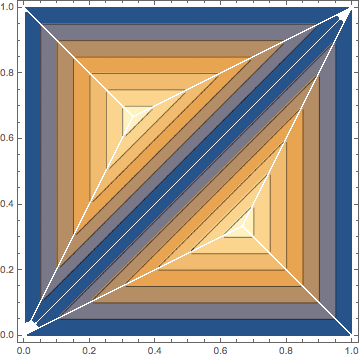
\includegraphics[width=1.5in]{3.png}
\centering
\end{figure}

لذا داریم:

\begin{center}
$
E(S)
= 6\Big( \int_{0}^{\frac{2}{3}} \int_{0}^{\frac{x}{2}} y\ dydx +\int_{\frac{2}{3}}^{1} \int_{0}^{1-x} y\ dydx  \Big)
=6\Big( \int_{0}^{\frac{2}{3}} \dfrac{x^2}{8}\ dx  + \int_{\frac{2}{3}}^{1} \dfrac{1}{2} - x + \dfrac{x^2}{2}\ dx\Big)
= \dots = 6\dfrac{1}{54} = \dfrac{1}{9}
$
\end{center}

و از آنجا که
$M = 1-L-S$،
لذا

\begin{center}
$E(M) = E(1-L-S) = 1-\dfrac{11}{18} - \dfrac{1}{9} = \dfrac{5}{18} $
\end{center}


\end{حل}

% ------------------------------------------------------
% problem 4
% ------------------------------------------------------
\newpage
\begin{prob}
\end{prob}

\begin{حل}
متغیر تصادفی
$R_n$
را برابر با تعداد رکوردشکنی‌ها تا لحظه مشاهده
$n$
نمونه در نظر می‌گیریم
\cite{andel}.
فرض کنیم متغیر تصادفی کمکی
$I_i$
عبارت باشد از آنکه متغیر تصادفی
$X_i$
یک رکورد باشد. یعنی

\begin{center}
$
I_i = \begin{cases}
1 & \text{$X_i$ یک رکورد است}\\
0 & \text{در غیر این صورت}
\end{cases}
$
\end{center}

در این صورت احتمال یک بودن
$I_i$
عبارت است از
اینکه در بین مقادیر (با احتمال یک متمایز)
$X_1, \dots, X_i$،
ماکسیمم در جایگاه
$i$ام
قرار بگیرد و بقیه مقادیر با هر ترتیب دلخواهی قرار داشته باشند. یعنی
$Pr[I_i=1] = \dfrac{1}{i}$.
در واقع پیشامد‌های آینده در لحظه مستقل از پیشامدهای گذشته هستند. یعنی

\begin{center}
$
Pr[I_i\ |\ X_1, \dots, X_n] = Pr[I_i\ |\ X_1,\dots ,X_i]
$
\bigbreak
$
Pr[I_i=1\ |\ X_1=x_1, \dots, X_n=x_n] = Pr[I_i=1\ |\ X_1=x_1, \dots, X_i=x_i] = \dfrac{1 \times (i-1)!}{i!} = \dfrac{1}{i}
$
\end{center}

اکنون توجه می‌کنیم که

\begin{center}
$
R_n = \sum_{i=1}^{n} I_i
\implies
E[R_n] = E[I_1 + \dots + I_n] 
= E[I_1] + \dots + E[I_n]
$
\bigbreak
$
= Pr[I_1=1] + \dots + Pr[I_n=1]
= \sum_{i=1}^{n} \dfrac{1}{i}
$
\end{center}

طبق
\cite{andel}،
اگر بخواهیم تقریبی برای
$E[R_n]$
بر اساس ثابت اویلر ($\gamma$) بدهیم، داریم:

\begin{center}
$
E[R_n] = \log n + \dfrac{1}{2n} + \dfrac{1}{12n^2} + \gamma + O(n^{-4})\..
$
\end{center}

\vspace*{1in}

اگر تعریف کنیم

\begin{center}
$
Y_n := \max \{ X_1,\dots ,X_n \},
\quad X_i \overset{iid}{\sim} \mathcal{N}(0, 1),
$
\end{center}

آنگاه طبق
\cite{max_Gaussian_bounds}،
ثابت می‌شود

\begin{center}
$
E[Y_n] = \theta (\sqrt{\log n})\..
$
\end{center}

در  واقع در
\cite{max_Gaussian_bounds}
نامساوی‌های زیر اثبات شده است که به ازای
$X_i$های
مستقل هم‌توزیع از یک توزیع نرمال با میانگین صفر و واریانس
$\sigma^2$
نمونه‌گیری شده‌اند.

\begin{center}
$
\dfrac{1}{\sqrt{\pi \log 2}} \sigma \sqrt{\log n} \leq E[Y_n] \leq \sqrt{2} \sigma \sqrt{\log n}
$
\end{center}

اثبات نامساوی کران پایین جزییات زیادی دارد که به طور کامل در
\cite{max_Gaussian_bounds}
ذکر شده است. تنها نامساوی کران بالا را اثبات می‌کنیم. به ازای
$t\geq 0$
ثابت، طبق نامساوی ینسن به ازای تابع محدب
$\exp: \mathbb{R} \rightarrow \mathbb{R}_{++}$
داریم:

\begin{center}
$
\exp(t E[Y_n]) \leq E[\exp(tY_n)]
= E[\exp(\max_{i \in \{1,\dots, n\}} tX_i)]
= E[\max_{i \in \{1,\dots, n\}} \exp(tX_i)]
$
\end{center}

اما متغیر تصادفی اندیکاتور
$I_{X_i}$
را به شکل زیر تعریف کنیم، نتیجه می‌شود:

\begin{center}
$
I_{X_i} = \begin{cases}
1 & X_i = Y_n\\
0 & X_i \neq Y_n
\end{cases} \qquad \implies \qquad
\max_{i \in \{1,\dots, n\}} \exp (tX_i)
= I_{X_1} \exp (tX_1) + \dots + I_{X_n} \exp (tX_n)
$
\end{center}

اما واضح است که

\begin{center}
$
E[I_{X_i}\exp(tX_i)] \leq E[\exp(tX_i)]
$
\end{center}

پس از ترکیب روابط بالا و استفاده از خاصیت خطی امید ریاضی، خواهیم داشت:

\begin{center}
$
\exp(tE[Y_n]) \leq 
E[\max_{i \in \{1,\dots, n\}} \exp(tX_i)]
= E[I_{X_1} \exp (tX_1) + \dots + I_{X_n} \exp (tX_n)]
$
\bigbreak
$
= E[I_{X_1} \exp (tX_1)] + \dots + E[I_{X_n} \exp (tX_n)]
\leq E[tX_1] + \dots + E[tX_n]
= nE[tX]
$
\end{center}

اکنون به ازای متغیر تصادفی نرمال
$X \sim \mathcal{N}(\mu, \sigma^2)$،
تابع مولد گشتاور
$E[\exp(tX)]$
عبارت است از
$\exp(\mu t + \dfrac{t^2 \sigma^2}{2})$.
لذا

\begin{center}
$
\exp (tE[Y_n]) \leq n\exp(\dfrac{t^2}{2})
\quad \implies \quad
tE[Y_n] \leq \log n + \dfrac{t^2}{2}
$
\end{center}

که با جایگذاری
$t:=\sqrt{2\log n}$
نامساوی کران بالا را نتیجه می‌دهد:

\begin{center}
$
E[Y_n] \leq \sqrt{2}\sqrt{\log n}
$
\end{center}

\end{حل}


% ------------------------------------------------------
% problem 5
% ------------------------------------------------------
\newpage
\begin{prob}
\end{prob}

\begin{حل}
ابتدا توجه می‌کنیم که با توجه به پارادوکس برتراند، نحوه نمونه‌گیری وترهای دایره می‌تواند متفاوت باشد و به نتایج متفاوتی منجر شود
\cite{bertrand_paradox}.
ما در اینجا فرض می‌کنیم یک وتر توسط میانه‌اش (به طور یکتا) مشخص شود. فرض کنیم دایره اصلی
$2r$
شعاع داشته باشد. در این صورت پیشامد اینکه وتر
$V \in \{(X,Y)\ |\ X^2+Y^2 \leq 4r^2\}$
با دایره کوچک درونی تلاقی داشته باشد، معادل است با اینکه مینیمم فاصله نقاط وتر با مرکز دایره اصلی، فاصله‌ای حداکثر برابر با
$r$
داشته باشد. اما فاصله وتر
$V$
با مرکز دایره اصلی همان فاصله نقطه
$V$
است. پس اگر نقطه میانه وتر را خارج از دایره کوچک انتخاب کنیم، هرگز با دایره کوچک تلاقی نخواهد داشت و برعکس. پس احتمال عدم تلاقی یک وتر تصادفی (نمونه‌گیری شده با روشی که فرض کردیم) عبارت است است از:

\begin{center}
$
\dfrac{\pi 4r^2 - \pi r^2}{\pi 4r^2} = \dfrac{3}{4}
$
\end{center}

در صورتی که دایره بزرگ‌تر با کوچک‌تر هم‌مرکز نباشد، نشان می‌دهیم این احتمال کاهش می‌یابد. ابتدا توجه می‌کنیم که در حالت کلی برای آنکه وتر داده شده
$V \in \{(X,Y)\ |\ X^2+Y^2 \leq 4r^2\}$
با دایره داخلی تلاقی نکند، بایست به ازای دو محل تلاقی دایره کوچک‌تر با خط موازی گذرنده از مرکز دایره کوچک‌تر
($O'$)
با خط
$OV$
(نقاط
$A'$
و
$B'$
در شکل زیر)، 
$V$
بیرون پاهای عمود این دو نقطه بر قطر
$OV$
قرار داشته باشد (بخش‌های سبز شده شکل زیر که به ازای یک قطر خاص با زاویه
$\theta$
با خط
$OO'$
رسم شده‌اند). در این خصوص به شکل زیر توجه می‌کنیم:

\bigbreak

\begin{figure}[h]
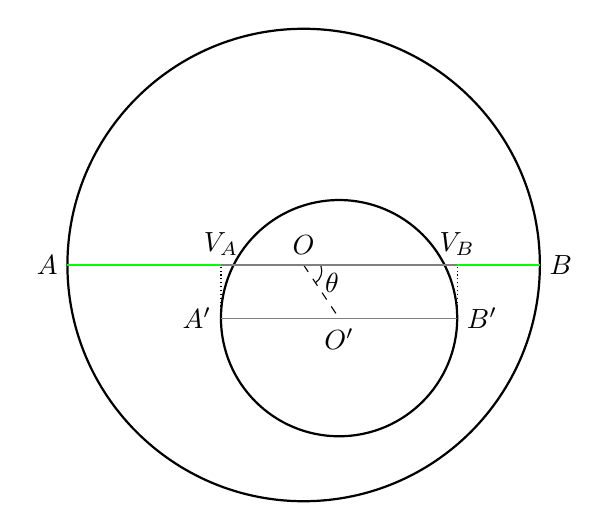
\begin{tikzpicture}[x=1cm, y=1cm, scale=1.5]
    \draw[thick] (0,0) circle (2cm) node[anchor=south] {$O$};
    \draw[thick] (0.3,-0.45)  circle (1cm) node[anchor=north] {$O'$};
    \draw[dashed] (0,0) -- (0.3,-0.45);
    \draw[-,color=green] (-2,0) -- (-0.7,0);
    \draw (-2,0) node[anchor=east] {$A$};
    \draw[-,color=gray] (-0.7,0) -- (1.3,0);
    \draw (2,0) node[anchor=west] {$B$};
    \draw[-,color=green] (1.3,0) -- (2,0);
    \draw[-,color=gray] (-0.7,-0.45) -- (1.3,-0.45);
    \draw (-0.7,-0.45) node[anchor=east] {$A'$};
    \draw (1.3,-0.45) node[anchor=west] {$B'$};
    \draw[densely dotted] (-0.7,-0.45) -- (-0.7,0) node[anchor=south] {$V_A$};
    \draw[densely dotted] (1.3,-0.45) -- (1.3,0) node[anchor=south] {$V_B$};
    \draw[] (0.1,-0.15) arc (-56.3:20:0.12);
    \draw (0.1,-0.15) node[anchor=west] {$\theta$};
\end{tikzpicture}
\centering
\end{figure}

آنچه در شکل فوق مورد توجه است، آن است که طول مجموع پاره‌خط سبز، هم‌چنان
$2r$
است، اما شامل دو تکه است که الزاما طول‌های برابر ندارند.

فرض کنیم به ازای
$\theta$
ثابت، طول
$OV_A$
را با
$x_{\theta}$
نشان دهیم. در این صورت مساحت ناحیه شامل همه مراکز وترهای تلاقی کننده با دایره داخلی عبارت است از:

\begin{center}
$
\int_{0}^{\pi} \int_{0}^{2r-x_{\theta}} s\ dsd\theta +
\int_{0}^{\pi} \int_{0}^{x_{\theta}} s\ dsd\theta 
= \int_{0}^{\pi} \dfrac{(2r-x_{\theta})^2}{2} \ d\theta +
\int_{0}^{\pi} \dfrac{x_{\theta}^2}{2}\ d\theta
= \pi r^2 + \int_{0}^{\pi} (r-x_{\theta})^2\ d\theta \geq \pi r^2
$
\end{center}

پس احتمال تلاقی وتر مذکور از
$\dfrac{\pi r^2}{4\pi r^2} = \dfrac{1}{4}$
بیشتر است و لذا احتمال عدم تلاقی کاهش می‌یابد. این کاهش بستگی به میزان
$r-x_{\theta}$
دارد و هرچه دایره کوچک‌تر به سمت مرزهای دایره بزرگ‌تر حرکت کند، احتمال عدم تلاقی وترها کاهش می‌یابد.


\end{حل}


% ------------------------------------------------------
% problem 6
% ------------------------------------------------------
\newpage
\begin{prob}
\end{prob}

\begin{حل}

مساله را در حالت کلی‌تر که سکه مورد نظر یک بیضی باشد حل می‌کنیم. فرض کنیم شعاع‌های بیضی مقادیر
$\alpha$
و
$\beta$
هستند که
$\beta \leq \alpha$.
هم‌چنین فرض کنیم مرکز بیضی مورد نظر به صورت
$(C_X,\ C_Y)$
باشد که مولفه‌ها به طور یکنواخت (بدون کاستن از کلیت مساله) از بازه
$[0,\ 3]$
انتخاب شده‌اند و بیضی تحت یک دوران به اندازه
$\theta$
درجه قرار گرفته باشد. پس هر بیضی نمونه‌گیری شده مطابق با فرض مساله، به صورت زیر به شکل یکتا در صفحه قرار می‌گیرد:

\begin{center}
$
\begin{cases}
C := (C_X,\ C_Y) \sim U[0, 3]^2 & \text{مختصات مرکز بیضی} \\
\theta \sim U[0,\pi] & \text{زاویه بین شعاع به طول $\alpha$ با محور افقی} 
\end{cases}
$
\end{center}

اگر معادله نقاط بیضی به صورت زیر باشد:

\begin{center}
$
f:\ ax^2 + bxy + cy^2 -d = 0
$
\end{center}

آنگاه دورترین خطوط افقی و عمودی که با این بیضی تلاقی می‌کنند، نقاطی است که در آنها مشتقات جزیی
$f$
نسبت به
$x$
و
$y$
برابر با صفر است. یعنی:

\begin{center}
$
\dfrac{\partial f}{\partial x} = 2ax + by = 0 
$

$
\implies x^* = \dfrac{-b}{2a}y^*
$

$
\implies a(\dfrac{b^2}{4a^2}){y^*}^2 + b(\dfrac{-b}{2a}){y^*}^2 + c{y^*}^2 - d = 0
$

$
\implies {y^*}^2 \big( \dfrac{b^2}{4a} - \dfrac{b^2}{2a} + c \big) = d
$

$
\implies {y^*}^2 (c - \dfrac{b^2}{4a}) = d
$

$
\implies {y^*}^2 = \dfrac{4ad}{4ac - b^2}
$
\end{center}

پس به طریقی مشابه، بعد از یافتن فرمول مشابهی برای مرزی‌ترین نقاط افقی بیضی مذکور، کلیه نقاط بیضی درون محدوده

\begin{center}
$
C_X \pm \sqrt{\dfrac{4cd}{4ac-b^2}}, \quad
C_Y \pm \sqrt{\dfrac{4ad}{4ac-b^2}}
$
\end{center}

قرار می‌گیرند.

اکنون توجه می‌کنیم که معادله نقاط بیضی هنگامی که زاویه شعاع به طول
$\alpha$
آن با محور افقی برابر با صفر باشد، به صورت زیر است:

\begin{center}
$
\dfrac{X^2}{\alpha ^2} + \dfrac{Y^2}{\beta ^2} = 1
$
\end{center}

اما معادله نقاط بیضی پس از دوران به اندازه
$\theta$
عبارت است از:
$R_{\theta} 
\begin{bmatrix}
X \\ Y
\end{bmatrix}
 = \begin{bmatrix}
 X_{\theta} \\ Y_{\theta}
 \end{bmatrix}
 $
 که در آن
 $R_{\theta}$
 ماتریس دو بعدی دوران مرسوم است. در نتیجه نقاط صادق در بیضی دوران یافته در معادلات زیر صدق می‌کنند:
 
\begin{center}
$
\begin{cases}
X = \cos \theta X_{\theta} + \sin \theta Y_{\theta} \\
Y = -\sin \theta X_{\theta} + \cos \theta Y_{\theta}
\end{cases}
$
\end{center}

که با جایگذاری در معادله اولیه، معادله بیضی دوران یافته به اندازه
$\theta$
به شکل زیر به دست می‌آید:

\begin{center}
$
\dfrac{(\cos \theta X_{\theta} + \sin \theta Y_{\theta})^2}{\alpha ^2} + \dfrac{(-\sin \theta X_{\theta} + \cos \theta Y_{\theta})^2}{\beta ^2} = 1
$
\end{center}

که اگر به فرم استاندارد مربعی معرفی شده در بالا آن را برگردانیم، عبارت است از:

\begin{center}
$
\implies X_{\theta}^2(\beta ^2 \cos^2 \theta + \alpha^2 \sin^2 \theta) + 
X_{\theta}Y_{\theta} (2\beta^2\sin \theta \cos \theta - 2\alpha^2 \sin \theta \cos \theta) + 
Y_{\theta}^2 (\beta^2\sin^2 \theta + \alpha^2 \cos^2 \theta) - \alpha^2 \beta^2 = 0
$
\end{center}

در نتیجه

\begin{center}
$
\implies 4ac - b^2 = 4 (\beta^4\cos^2 \theta \sin^2 \theta + \beta^2\alpha^2 \cos^4 \theta + \alpha^2 \beta^2\sin^4 \theta + \alpha^4 \sin^2 \theta \cos^2 \theta) - 4\sin^2 \theta \cos^2 \theta (\beta^4 -2\beta^2\alpha^2 + \alpha^4)
$

$
= 4 \alpha^2\beta^2 (\sin^4 \theta + \cos^4 \theta + 2\sin^2 \theta \cos^2 \theta) = 4\alpha^2 \beta^2
$
\end{center}

که نتیجه می‌دهد:

\begin{center}
$
X_{\theta, \max} = \sqrt{\alpha^2 \cos^2 \theta + \beta^2\sin^2 \theta}, \qquad
Y_{\theta, \max} = \sqrt{\alpha^2 \sin^2 \theta + \beta^2\cos^2 \theta}
$
\end{center}

پس به ازای
$\theta$
ثابت، تنها در صورتی بیضی مورد نظر با خطوط مشبکه تلاقی نمی‌کند که کاملا درون مستطیل به عرض
$3-2Y_{\theta, \max}$
و
طول
$3-2X_{\theta, \max}$
هاشور خورده در شکل زیر قرار بگیرد.

\bigbreak

\begin{figure}[h]
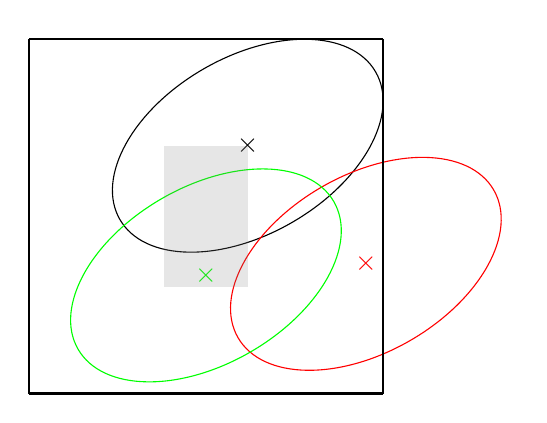
\begin{tikzpicture}[x=1cm, y=1cm, scale=1.5]
    \draw[rotate around={30:(1.854,2.098)}] (1.854,2.098) ellipse (1.25cm and 0.75cm);
    \node at (1.854,2.098) {$\times$};
    \draw[rotate around={30:(2.854,1.098)},red] (2.854,1.098) ellipse (1.25cm and 0.75cm);
    \node[red] at (2.854,1.098) {$\times$};
    \draw[rotate around={30:(1.5,1)},green] (1.5,1) ellipse (1.25cm and 0.75cm);
    \node[green] at (1.5,1) {$\times$};
    \draw[thick] (0,0) -- (3,0);
    \draw[thick] (3,0) -- (3,3);
    \draw[thick] (3,3) -- (0,3);
    \draw[thick] (0,3) -- (0,0);
    \fill [gray,fill opacity=0.2] (1.145,0.901) rectangle (1.854,2.098);
\end{tikzpicture}
\centering
\end{figure}

اگر پیشامد قرار گرفتن بیضی در داخل یک مربع را
$I_{\theta}$
بنامیم، از آنچه در شکل بالا نشان داده شد به دست می‌آید که (با فرض برابر بودن طول ضلع هر مربع با مقدار
$l$):

\begin{center}
$
Pr[I_{\theta}\ |\ \theta] = \dfrac{1}{l^2} (l-2 X_{\theta, \max}) (l- 2Y_{\theta, \max})
$
\end{center}

به دلیل تقارن موجود، مقادیر
$\theta$
را می‌توان به
$[0, \dfrac{\pi}{2}]$
محدود کرد. به کمک قانون احتمال کل داریم:

\begin{center}
$
Pr[I] = \dfrac{2}{\pi}\int_{0}^{\frac{\pi}{2}} Pr[I_{\theta}\ |\ \theta]\, d\theta
$
\bigbreak
$
= \dfrac{2}{\pi} \int_{0}^{\frac{\pi}{2}} 1 - \dfrac{2}{l} (X_{\theta, \max} + Y_{\theta, \max}) + \dfrac{4}{l^2} X_{\theta, \max} Y_{\theta, \max} \, d\theta
$
\end{center}

اما به کمک تابع انتگرال بیضوی
$K(m)$
با ضابطه زیر
\cite{ellipk}،

\begin{center}
$
K(m) := \int_{0}^{\frac{\pi}{2}} \sqrt{1-m\sin ^2(t)}\, dt
$
\end{center}

می‌توان انتگرال‌های فوق را ساده‌سازی کرد:

\begin{center}
$
\int_{0}^{\frac{\pi}{2}} X_{\theta, \max}\, d\theta
= \int_{0}^{\frac{\pi}{2}} Y_{\theta, \max} \, d\theta
= \int_{0}^{\frac{\pi}{2}} \sqrt{\alpha^2 \cos^2 \theta + \beta^2 \sin^2 \theta}\, d\theta
= \alpha K(1-(\dfrac{\beta}{\alpha})^2)
$
\bigbreak
$
\int_{0}^{\frac{\pi}{2}} X_{\theta, \max}Y_{\theta, \max}\, d\theta 
= \int_{0}^{\frac{\pi}{2}} \sqrt{\Big(\alpha^2 - \sin^2 \theta (\alpha^2 - \beta^2)\Big) \Big( \beta^2 + \sin^2 \theta (\alpha^2 - \beta^2) \Big)} \, d\theta 
$
\bigbreak
$
=\int_{0}^{\frac{\pi}{2}}\sqrt{\alpha^2 \beta^2 -(\alpha^2 - \beta^2)^2 (\sin^4 \theta - \sin^2 \theta}) \, d\theta
=\int_{0}^{\frac{\pi}{2}}\sqrt{\alpha^2 \beta^2 +\dfrac{1}{4}(\alpha^2 - \beta^2)^2 \sin^2 2\theta} \, d\theta
$
\bigbreak
$
=\dfrac{1}{2}\int_{0}^{\frac{\pi}{2}}\sqrt{4\alpha^2 \beta^2 +(\alpha^2 - \beta^2)^2 \sin^2 \theta} \, d\theta
= \dfrac{\alpha^2 + \beta^2}{2} K\Big( (\dfrac{\alpha^2 - \beta^2}{\alpha^2 + \beta^2})^2 \Big)
$
\end{center}

و با جایگذاری در معادله اصلی داریم:

\begin{center}
$
Pr[I] = 1 - \dfrac{8\alpha}{l\pi} K\Big( 1-(\dfrac{\beta}{\alpha})^2 \Big) + 
\dfrac{4(\alpha^2 + \beta^2)}{l^2\pi} K\Big( (\dfrac{\alpha^2 - \beta^2}{\alpha^2 + \beta^2})^2 \Big)
$
\end{center}

برای حالتی که بیضی مورد نظر یک دایره باشد نیز، داریم:

\begin{center}
$
\alpha=\beta \implies Pr[I] = 1 - \dfrac{8\alpha}{l\pi}K(0) + \dfrac{8\alpha^2}{l^2\pi}K(0)
\quad \overset{K(0)=\frac{\pi}{2}}{\implies} \quad
Pr[I] = (1-\dfrac{2\alpha}{l})^2
$
\end{center}

اکنون به مساله بر می‌گردیم. حالات زیر سوال شده بودند که مقدار هر یک را به دست آورده‌ایم:

\begin{LTR}
\begin{itemize}
\item{
$
\alpha = \beta = 1:\
Pr[I] = (1-\dfrac{2}{3})^2 = \dfrac{1}{9}
$
}
\item{
$
\alpha=\dfrac{5}{4}, \beta=\dfrac{3}{4}\
Pr[I] = 1 - \dfrac{10}{3\pi} K(\dfrac{16}{25}) + \dfrac{17}{18\pi} K(\dfrac{64}{289}) 
$
}
\end{itemize}
\end{LTR}

به ازای بیضی با قطرهای
$2.5$
و
$1.5$، مقدار به دست آمده به کمک شبیه‌سازی تقریبا برابر با
$0.0907$
است. نکته قابل توجه آنکه با وجود مساحت کمتر بیضی مذکور ($
\dfrac{15}{16} \pi
$)
 نسبت به دایره واحد ($
\pi
$)،
احتمال عدم تلاقی بیضی با مرز‌ها کمتر است.

در شکل زیر نقاط مرکز بیضی‌های با قطرهای مشخص شده فوق، با یک دوران تصادفی در نظر گرفته شده‌اند و در صورتی که بیضی دوران یافته با مرزها تلاقی نکرده باشد، با رنگ آبی رنگ‌آمیزی شده‌اند.

\begin{figure}[h]
\subfloat[]{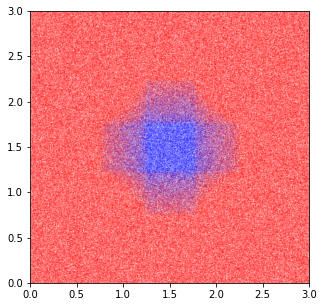
\includegraphics[width = 2in]{6.png}} 
\subfloat[]{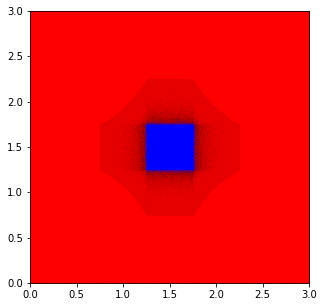
\includegraphics[width = 2in]{6_b.png}} 
\label{6}
\centering
\end{figure}

\end{حل}


% ------------------------------------------------------
% problem 7
% ------------------------------------------------------
\newpage
\begin{prob}
\end{prob}

\begin{حل}
\end{حل}


% ------------------------------------------------------
% problem 8
% ------------------------------------------------------
\newpage
\begin{prob}
\end{prob}

\begin{حل}

ماتریس انتقال فرآیند مارکف مساله به شکل زیر است:

\begin{center}
$
P = 
\begin{bmatrix}
0 & \dfrac{1}{2} & 0& \dfrac{1}{2}\\
\dfrac{1}{3} & 0 & \dfrac{1}{3} & \dfrac{1}{3}\\
0& \dfrac{1}{2} & 0 & \dfrac{1}{2}\\
\dfrac{1}{3} & \dfrac{1}{3} & \dfrac{1}{3} & 0\\
\end{bmatrix}
$
\end{center}

به این ترتیب اگر
$\sigma^{(n)}$
بردار احتمال حضور قدم‌زن تصادفی بعد از
$n$
گام در هر راس باشد، داریم

\begin{center}
$
\begin{cases}
\sigma^{(n)} = \sigma^{(n-1)}P = \sigma^{(0)}P^n & \qquad n \geq 1\\
\sigma^{(0)} = (1, 0, 0, 0)
\end{cases}
$
\end{center}

می‌دانیم در درازمدت، بردار
$\sigma^{(n)}$
به توزیع پایای
$\pi$
میل می‌کند و در واقع تغییر زیادی نمی‌کند. پس از یک زمانی مثل
$N$
به بعد، احتمال حضور در راس
$B$
در گام
$n\geq T$
تقریبا برابر است با
$\pi_2$.
پس به طور متوسط با احتمال تقریبا
$\pi_2$
در یک لحظه تصادفی ولی به اندازه کافی طولانی، در راس
$B$
قرار داریم. پس به دنبال بردار
$\pi$
می‌گردیم.
داریم:

\begin{center}
$
\pi P = pi
\implies \pi (P-I) = 0
\implies (P^T-I)\pi^T = 0
$
\end{center}

پس به دنبال برداری (با مجموع درایه‌های برابر با یک) هستیم که در کرنل ماتریس
$P^T-I$
قرار داشته باشد. به کمک عکلیات سطری مقدماتی، خواهیم داشت:

\begin{center}
$
P^T-I
=
\begin{bmatrix}
-1 & \dfrac{1}{3} & 0 & \dfrac{1}{3}\\
\dfrac{1}{2} & -1 & \dfrac{1}{2} & \dfrac{1}{3}\\
0 & \dfrac{1}{3} & -1 & \dfrac{1}{3}\\
\dfrac{1}{2} & \dfrac{1}{3} & \dfrac{1}{2} & -1
\end{bmatrix}
\ \rightarrow \
\begin{bmatrix}
1 & -\dfrac{1}{3} & 0 & -\dfrac{1}{3}\\
0 & -\dfrac{5}{6} & \dfrac{1}{2} & \dfrac{1}{2}\\
0 & \dfrac{1}{3} & -1 & \dfrac{1}{3}\\
0 & \dfrac{1}{2} & \dfrac{1}{2} & -\dfrac{5}{6}
\end{bmatrix}
\ \rightarrow \
\begin{bmatrix}
1 & 0 & \dfrac{1}{3} & -\dfrac{8}{9}\\
0 & 1 & 1 & -\dfrac{5}{3}\\
0 & 0 & -\dfrac{4}{3} & \dfrac{8}{9}\\
0 & 0 & \dfrac{4}{3} & -\dfrac{8}{9}
\end{bmatrix}
\ \rightarrow \
\begin{bmatrix}
1 & 0 & 0 & -\dfrac{2}{3}\\
0 & 1 & 0 & -1\\
0 & 0 & 1 & -\dfrac{2}{3}\\
0 & 0 & 0 & 0
\end{bmatrix}
$
\end{center}

که نتیجه می‌دهد:

\begin{center}
$
\begin{cases}
\pi_A - \dfrac{2}{3}\pi_D = 0\\
\pi_B - \pi_D = 0\\
\pi_C - \dfrac{2}{3}\pi_D = 0\\
\pi_A + \pi_B + \pi_C + \pi_D = 1
\end{cases}
\qquad \implies \qquad
\pi = (\dfrac{2}{10}, \dfrac{3}{10}, \dfrac{2}{10}, \dfrac{3}{10})
$
\end{center}

پس به طور میانگین قدم‌زن تصادفی در
$30\%$
اوقات در راس
$B$
قرار دارد.

\vspace*{1in}

اکنون اگر یال‌های گراف را جهت‌دار در نظر بگیریم و یال‌های خروجی از
$C$
را حذف کنیم، بردار
$\sigma_C^{(n)}$
که مشابه قبل برای این زنجیر مارکف جدید تعریف شود، هم‌چنان احتمال حضور در راس‌ها را در گام
$n$ام
قدم‌زن تصادفی نمایش می‌دهد. با این نکته که اگر قدم‌زن به راس
$C$
وارد شود، دیگر امکان خروج از آن را ندارد. پس متغیرهای تصادفی اندیکاتور زیر را تعریف می‌کنیم:

\begin{center}
$
I_n :=
\begin{cases}
1 & \qquad \text{قدم‌زن در لحظه $n$ام در راس $C$ قرار دارد}\\
0 & \qquad \text{در غیر این صورت}
\end{cases}
$
\end{center}

هم‌چنین پیشامد آنکه تا لحظه
$n$ام
راس
$C$
را دیده باشیم برابر با
$U_n$
تعریف می‌کنیم. داریم:

\begin{center}
$
Pr[U_n] = Pr[I_0 = 1] + \sum_{i=1}^{n}Pr[I_i=1\ |\ I_{i-1}=0]
= \sum_{i=1}^{n} Pr[I_i=1\ |\ I_{i-1}=0]
= \sum_{i=1}^{n} (\sigma_C^{(i)})_3 - (\sigma_C^{(i-1)})_3
= (\sigma_C^{(n)})_3
$
\bigbreak
$
= \sigma_C^{(0)} P_C^n \begin{pmatrix}
0 & 0 & 1 & 0
\end{pmatrix}^T
= \begin{pmatrix}
1 & 0 & 0 & 0
\end{pmatrix}
P_C^n \begin{pmatrix}
0 \\ 0 \\ 1 \\ 0
\end{pmatrix}
$
\end{center}

پس ابتدا چندجمله‌ای مشخصه ماتریس
$P_C$
را به دست می‌آوریم:

\begin{center}
$
P_C = 
\begin{bmatrix}
0 & \dfrac{1}{2} & 0& \dfrac{1}{2}\\
\dfrac{1}{3} & 0 & \dfrac{1}{3} & \dfrac{1}{3}\\
0& 0 & 1 & 0\\
\dfrac{1}{3} & \dfrac{1}{3} & \dfrac{1}{3} & 0\\
\end{bmatrix}
\qquad \implies \qquad \det(P_C - \lambda I) = \lambda^4 - \lambda^3 - \dfrac{4}{9}\lambda^2 + \dfrac{1}{3}\lambda + \dfrac{1}{9}
$
\end{center}

لذا مقادیر ویژه ماتریس
$P_C$
عبارتند از


\begin{center}
$
\lambda_1 = 1,\quad 
\lambda_2 = -\dfrac{1}{3},\quad 
\lambda_3 = \dfrac{1 + \sqrt{13}}{6},\quad 
\lambda_4 = \dfrac{1 - \sqrt{13}}{6}
$
\end{center}

اما از آنجا که یک ترکیب خطی از این مقادیر، همان
$Pr[U_n]$
خواهد بود، سعی می‌کنیم ضرایب ترکیب خطی را با تشکیل دستگاه معادلات خطی به دست آوریم:

\begin{center}
$
Pr[U_n] := a\lambda_1^n + b\lambda_2^n + c\lambda_3^n + d\lambda_4^n
$
\bigbreak
$
\begin{cases}
Pr[U_0] = 0 \\
Pr[U_1] = 0 \\
Pr[U_2] = \dfrac{1}{3}\\
Pr[U_3] = \dfrac{4}{9}
\end{cases}
\qquad \implies \qquad
\begin{bmatrix}
1 & 1 & 1 & 1\\
1 & \lambda_2 & \lambda_3 & \lambda_4\\
1 & \lambda_2^2 & \lambda_3^2 & \lambda_4^2\\
1 & \lambda_2^3 & \lambda_3^3 & \lambda_4^3\\
\end{bmatrix}
\begin{bmatrix}
a \\ b \\ c \\ d
\end{bmatrix} = 
\begin{bmatrix}
0 \\ 0 \\ \dfrac{1}{3} \\ \dfrac{4}{9}
\end{bmatrix}
$
\end{center}

با حل دستگاه خطی فوق به دست می‌آید:

\begin{center}
$
Pr[U_n] = 1 + (\dfrac{-5\sqrt{13} - 13}{26})(\dfrac{1 + \sqrt{13}}{6})^n +  (\dfrac{5\sqrt{13} - 13}{26})(\dfrac{1 - \sqrt{13}}{6})^n
$
\end{center}

پس احتمال آنکه تا لحظه
$n$ام
راس
$C$
را نبینیم برابر است با
$1-Pr[U_n]$
که مقدار دقیق آن از رابطه بالا قابل محاسبه است.


\end{حل}

% ------------------------------------------------------
% problem 9
% ------------------------------------------------------
\newpage
\begin{prob}
\end{prob}

\begin{حل}

اگر امید ریاضی زمانی که طول می‌کشد تا از راس
$X$
به
$Y$
برسیم را با
$T_{X,Y}$
نشان دهیم، روابط زیر نتیجه می‌شوند:

\begin{center}
$
\begin{cases}
T_{A,B} = p\times 1 + (1-p)\times (T_{C, B}+1) & = 1 + (1-p)T_{C,B}\\
\dots\\
T_{C,B} = (1-r)\times 1 + r\times (T_{A, B}+1) & = 1 + rT_{A,B}\\
\end{cases}
$
\end{center}

با مرتب کردن این معادلات خطی، معادله ماتریسی زیر را خواهیم داشت:

\begin{center}
$
\begin{bmatrix}
1 & 0 & 0 & 0 & 0 & p-1\\
0 & 1 & 0 & -q & 0 & 0\\
0 & 0 & 1 & 0 & -p & 0\\
0 & r-1 & 0 & 1 & 0 & 0\\
0 & 0 & q-1 & 0 & 1 & 0\\
-r & 0 & 0 & 0 & 0 & 1
\end{bmatrix}
\begin{bmatrix}
T_{A, B}\\
T_{B, A}\\
T_{A, C}\\
T_{C, A}\\
T_{B, C}\\
T_{C, B}
\end{bmatrix}
 = 
 \begin{bmatrix}
 1 \\ 1\\ 1\\ 1\\ 1\\ 1
 \end{bmatrix}
$
\end{center}

با حل دستگاه فوق به کمک روش سطری مقدماتی نتیجه می‌شود:

\begin{center}
$
(T_{A, B}, T_{B, C}, T_{C, A}) = \Big( 
\dfrac{2 - p}{1-r+rp},\ 
\dfrac{2-q}{1-p+pq},\ 
\dfrac{2-r}{1-q+qr}
\Big)
$
\bigbreak
$
(T_{A,C}, T_{C,B}, T_{B,A}) = \Big(
\dfrac{1+p}{1-p+pq},\ 
\dfrac{1+r}{1-r+rp},\ 
\dfrac{1+q}{1-q+qr}
\Big)
$
\end{center}

پس اختلاف میانگین زمانی که طول می‌کشد تا یک دور مثلثاتی بزنیم با میانگین زمانی که طول می‌کشد تا یک دور در خلاف جهت مثلثاتی بزنیم، برابر است با

\begin{center}
$
T_{diff}=
\dfrac{1-r-p}{1-r+rp} + 
\dfrac{1-p-q}{1-p+pq} +
\dfrac{1-r-q}{1-q+qr}
$
\end{center}

اگر کمیت
$T_{diff}$
منفی باشد، یعنی به طور متوسط زمانی که طول می‌کشد تا یک دور مثلثاتی بزنیم، کمتر است. پس در درازمدت در جهت مثلثاتی خواهیم چرخید.

\begin{center}
$
\begin{cases}
T_{diff} < 0 & \text{در درازمدت در جهت مثلثاتی خواهیم چرخید.}\\
T_{diff} = 0 & \text{در درازمدت در هیچ جهتی نمی‌چرخیم.}\\
T_{diff} > 0 & \text{در درازمدت در خلاف جهت مثلثاتی خواهیم چرخید.}
\end{cases}
$
\end{center}

برای یافتن سرعت نیز، فرض کنیم
$T^+ := T_{A,B} + T_{B,C} + T_{C,A}$
و
$T^- := T_{A,C} + T_{C,B} + T_{B,A}$.
در این صورت در یک واحد زمانی به طور متوسط،
$\dfrac{1}{T^+}$
از کمان
$[0,\ 2\pi]$
را در جهت مثلثاتی طی کرده‌ایم و
$\dfrac{1}{T^-}$
از کمان فوق را در خلاف جهت مثلثاتی طی کرده‌ایم. پس به طور میانگین در هر واحد زمانی به میزان
$\dfrac{1}{T^+} - \dfrac{1}{T^-}$
از کمان
$[0,\ 2\pi]$
را در جهت مثلثاتی طی کرده‌ایم. این مقدار طبق تعریف، سرعت حرکت در جهت مثلثاتی خواهد بود (توجه می‌کنیم که می‌تواند مقادیر آن مثبت یا منفی شود).

\begin{center}
$
V^+ 
=\dfrac{T^- - T^+}{T^+ T^-}
= -\dfrac{T_{diff}}{T^+ T^-}
$
\end{center}

\end{حل}

% ------------------------------------------------------
% problem 10
% ------------------------------------------------------
\newpage
\begin{prob}
\end{prob}

\begin{حل}

اگر زمانی که طول می‌کشد تا تعداد افراد مبتلا از
$k-1$
نفر به
$k$
نفر برسد را
$T_k$
بنامیم و احتمال ابتلای یک فرد جدید را زمانی که تعداد مبتلایان
$k-1$
نفر است،
$p_k$
بنامیم،  داریم:

\begin{center}
$
p_k = p\times \dfrac{
\begin{pmatrix}
k-1 \\ 1
\end{pmatrix}
\begin{pmatrix}
n-k+1 \\ 1
\end{pmatrix}
}{
\begin{pmatrix}
n \\ 2
\end{pmatrix}
} 
= p\dfrac{2(k-1)(n-k+1)}{n(n-1)}, \qquad k\geq 2
$
\bigbreak
$
E[T_k] = \sum_{i=1}^{\infty} i p_k(1-p_k)^{i-1}
= p_k \times \dfrac{d (\sum_{i=0}^{\infty}x^i)}{d x}\Big|_{1-p_k}
= p_k \times \dfrac{1}{(1-x)^2}\Big|_{x=1-p_k}
= \dfrac{1}{p_k}
$
\end{center}

پس امید ریاضی مجموع زمان لازم برای ابتلای همه افراد شهر برابر است با

\begin{center}
$
E[T_2 + \dots + T_n] = \sum_{k=2}^{n}  E[T_k] = \sum_{k=2}^{n} \dfrac{1}{p_k} = \sum_{k=2}^{n} \dfrac{\begin{pmatrix}
n\\ 2
\end{pmatrix}}{
p (k-1) (n-k+1)
}
$
\bigbreak
$
= \dfrac{\begin{pmatrix}
n\\2
\end{pmatrix}
}{p} \sum_{k=2}^{n}\dfrac{1}{(k-1)(n-k+1)}
= \dfrac{\begin{pmatrix}
n\\2
\end{pmatrix}
}{p} \sum_{k=2}^{n}\dfrac{1}{n} \Big( \dfrac{1}{k-1} + \dfrac{1}{n-k+1}\Big)
= \dfrac{n-1}{p} \sum_{k=1}^{n-1} \dfrac{1}{k}
= \theta (\dfrac{1}{p} n^2 \log n)
$
\end{center}


\end{حل}

% ------------------------------------------------------
% problem 11
% ------------------------------------------------------
\newpage
\begin{prob}
\end{prob}

\begin{حل}
\end{حل}
% ------------------------------------------------------
% problem 12
% ------------------------------------------------------
\newpage
\begin{prob}
\end{prob}

\begin{حل}
\end{حل}





















% ------------------------------------------------------
% problem 13
% ------------------------------------------------------
\newpage
\begin{prob}
\end{prob}

\begin{حل}
مساله الکسی ایوانویچ را در حالت کلی که
$n$
واحد پول داشته باشد و با احتمال
$p$
$(p \leq \dfrac{1}{2})$
بتواند نتیجه پرتاب سکه را درست حدس بزند، حل می‌کنیم. پس فرض کنیم الکسی به دنبال برنده شدن مجموعا
$2n$
واحد پول است و از طرفی اگر پولش صفر شود، باید از بازی خارج شود.

نشان خواهیم داد بیشترین شانس الکسی هنگامی رخ می‌دهد که وی همه
$n$
سکه خود را یکجا شرط بندی کند. سپس در حالت کلی‌تر که الکسی به دنبال برنده شدن مجموعا
$n+m$
واحد پول است، پیشنهادی برای بهترین روش عمل الکسی ارایه می‌کنیم.


فرض پیشامد برنده شدن الکسی (دریافت
$n$
واحد پول جدید و خروج از بازی با
$2n$
واحد در مجموع)
را با
$Q_{win}$
نشان دهیم و پیشامد باختن الکسی (از دست
$n$
واحد پول خودش و خروج با
$0$
واحد پول در مجموع) را با
$Q_{lose}$
نشان دهیم. چون تنها اتفاقاتی که منجر به تمام شدن بازی می‌شوند، بردن یا باختن الکسی است، و در زمان متناهی به یکی از این دو اتفاق جاذب در زنجیر مارکف می‌رسیم، پس:

\begin{center}
$
Pr[Q_{win}] + Pr[Q_{lose}] = 1
$
\end{center}

در حالتی که الکسی همه پولش را یکجا شرط‌بندی کند، طبق مفروضات مساله داریم:

\begin{center}
$
Pr[Q_{win}] = p,
\qquad 
Pr[Q_{lose}] = 1-p
\..
$
\end{center}

اکنون نشان می‌دهیم که در صورتی که الکسی هر بار با یک واحد پول شرط‌بندی کند، شانس بردنش کاهش می‌یابد. برای این کار فرض کنیم
$Z_i$
متغیر تصادفی تعداد واحد پول برده یا باخته الکسی در شرط بندی
$i$ام
باشد. در این صورت:

\begin{center}
$
Z_i = 
\begin{cases}
1
&
\text{الکسی با احتمال
$p$
نتیجه پرتاب سکه
$i$ام
را درست پیش‌بینی کرده است.}
\\
-1
&
\text{الکسی با احتمال
$1-p$
نتیجه پرتاب سکه
$i$ام
را اشتباه پیش‌بینی کرده است.}
\end{cases}
$
\end{center}

به علاوه، متغیرهای تصادفی
$S_k = \sum_{i=1}^{k} Z_i$
و
$T$
را به ترتیب برابر با مجموع پول برده یا باخته الکسی تا بازی
$k$ام
و زمان کل بازی تا رخ دادن یکی از پیشامدهای
$Q_{win}$
یا
$Q_{lose}$
در نظر می‌گیریم. در این صورت
$S_T$
شامل دو رخداد بردن یا باختن الکسی است و اگر
$Pr[Q_{win}|T]$
را برابر با
$q_T$
تعریف کنیم، داریم:

\begin{center}
$
Pr[S_T = n] = Pr[Q_{win}|T] = q_T,
\qquad 
Pr[S_T = -n] = Pr[Q_{lose}|T] = 1-q_T
\..
$
\end{center}

اکنون از تساوی والد
\cite{wald_wiki}
نتیجه می‌شود:

\begin{center}
$
E(T)E(Z) = E(S_T) 
\implies 
E(T)
\big( 1\times p + (-1) \times (1-p) \big) 
=
n \times q_T + (-n) \times (1-q_T)
$

$
\implies
E(T) (2p-1) = n(2q_T-1)
$
\end{center}

از طرفی چون در هر گام حداکثر می‌توان یک واحد پول برنده شد، برای برنده شدن
$n$
واحد پول حداقل می‌بایست
$n$
بار بازی کنیم و این یعنی
$E(T) \geq n$.
پس

\begin{center}
$
E(T) \geq n
\implies
E(T)(2p-1) \leq n(2p-1)
\implies
n(2q_T-1) \leq n(2p-1)
\implies q_T \leq p
$
\end{center}

توجه می‌کنیم که در نامساوی بالا، از نامثبت بودن
$2p-1$
یا معادلا از
$p\leq \dfrac{1}{2}$
استفاده شد و اگر
$p\geq \dfrac{1}{2}$،
جهت نامساوی آخر عکس می‌شود. یعنی اگر الکسی قدرت پیش‌بینی نتیجه پرتاب سکه را بهتر از پیش‌بینی تصادفی داشته باشد، بهتر است که به جای یک بازی، بازی‌های یک واحدی انجام دهد و برعکس اگر قدرت پیش‌بینی او (حالت منطقی‌تر) حداکثر تصادفی باشد، بهتر است به یکباره کل سرمایه خود را بازی کند.

\bigbreak

در حالت کلی‌تر زیر نیز نشان می‌دهیم که نتایج بالا هم‌چنان برقرارند. فرض کنیم الکسی در هر بازی خود، تعداد
$r$
واحد پول را با احتمال
$w_r$
بازی کند (در این حالت فرض کرده‌ایم الکسی همواره بتواند تا
$n$
واحد بازی کند، یعنی امکان قرض گرفتن موقت کمی پول را داشته باشد
). در این صورت متغیر تصادفی
$Z_i$
به شکل زیر تعمیم می‌یابد:

\begin{center}
$
Z_i = 
\begin{cases}
n
&
\text{الکسی با احتمال
$w_np$
در بازی
$i$ام
برنده
$n$
واحد پول شده است.}
\\
n-1
&
\text{الکسی با احتمال
$w_{n-1}p$
در بازی
$i$ام
برنده
$n-1$
واحد پول شده است.}
\\
\vdots
\\
-n + 1
&
\text{الکسی با احتمال
$w_{n-1}(1-p)$
در بازی
$i$ام
$n-1$
واحد پول باخته است.}
\\
-n
&
\text{الکسی با احتمال
$w_n(1-p)$
در بازی
$i$ام
$n$
واحد پول باخته است.}
\end{cases}
$
\end{center}

در این صورت مشابه قسمت قبل داریم

\begin{center}
$
E(T)E(Z) = E(S_T) 
\implies
E(T) \big( \sum_{k=1}^{n} (kw_k p + (-k)w_k(1-p)) \big) = n(2q_T-1)
$
\bigbreak
$
\implies
E(T)(2p-1)\sum_{k=1}^{n} kw_k = n(2q_T-1)
$
\end{center}

اما کمیت
$\sum_{k=1}^{n}kw_k$
برابر است با امید ریاضی تعداد واحد پول‌هایی که الکسی در هر بازی شرط‌بندی می‌کند. یا به عبارت دیگر، متوسط پولی که الکسی در هر بازی وارد می‌کند. پس
$E(T)\sum_{k=1}^{n}kw_k$
عبارت است از متوسط پولی که الکسی در مجموع تا رسیدن به
حالت باخت کامل یا برد کامل بازی کرده است و واضح است که این مقدار حداقل برابر با
$n$
است. پس

\begin{center}
$
E(T) \sum_{k=1}^{n}kw_k \geq n
\implies 
E(T) \sum_{k=1}^{n}kw_k (2p-1) \leq n (2p-1)
$

$
\implies 
n(2q_T-1) \leq n(2p-1)
\implies
q_T \leq p
$
\end{center}

توجه می‌کنیم که شرط امکان قرض گرفتن پول توسط الکسی، به نفع او بود و اگر شرط را بر داریم،
$q_T$
کاهش می‌یابد. پس به طور کلی نشان دادیم اگر الکسی قدرت ویژه‌ای در پیش‌بینی نتیجه پرتاب سکه ندارد، بهترین استراتژی او بازی یکباره کل پولش در همان مرحله اول است.

\bigbreak

در درس یادگیری تقویتی دکتر علیشاهی
\cite{alishahi_RL}، 
این مساله بررسی شده است و بهترین استراتژی در آنجا، بازی کردن تعداد واحد پولی بود که هر چه سریع‌تر بازی به اتمام برسد. یعنی رساندن کل پول قمارباز به عددی که پس از آن با ریسک کردن کل پول، هر بار امید به دو برابر شدنش داشته باشیم تا نهایتا کل پولی که به دنبالش هستیم برنده شویم. همانطور که در بالا مشاهده کردیم، نتایج ما با این مشاهدات سازگار هستند.

\end{حل}




% ------------------------------------------------------
% problem 14
% ------------------------------------------------------
\newpage
\begin{prob}
مساله فرآیند پواسون تصادفات جاده‌ای را بررسی می‌کنیم. اگر اطلاعات زیر را داشته باشیم، به دنبال احتمال پیشامد بروز تعدادی تصادف رانندگی در ماه آینده هستیم که هیچ‌کدام مرگبار نباشند.

\begin{center}
$
\begin{cases}
X_i &
\text{پیشامد بروز تصادف
$i$ام
در ماه
}
\\
Y_i &
\text{پیشامد مرگبار بودن تصادف
$i$ام}
\\
N &
\text{متغیر تصادفی تعداد تصادفات رانندگی در یک ماه}
\end{cases}
\implies
\begin{cases}
E(N) = 3\\
Pr[Y_i=1\ |\ X_i=1] = \dfrac{1}{3}
\end{cases}
$
\end{center}
\end{prob}

\begin{حل}

از آنجا که تصادفات جاده‌ای یک فرآیند پواسون است، طبق تعریف، تعداد تصادفات در یک بازه زمانی مشخص (یک ماهه) توزیع پواسون خواهد داشت. از طرفی طبق فرض مساله،
$E(N) = 3$،
و لذا
$N \sim Poisson (3)$.

پس داریم

\begin{center}
$
Pr[N = n] = \dfrac{3^n e^{-3}}{n!}
$
\end{center}

اکنون محاسبات زیر را داریم:

\bigbreak

\begin{LTR}
$
Pr[\text{تعداد مثبتی تصادف رخ دهد و هیچ کدام مرگبار نباشند}]
$
\bigbreak
$
= Pr[\cup_{n=1}^{\infty} \text{$n$ تصادف رخ دهد و هیچ کدام مرگبار نباشند}]
$
\bigbreak
$
= \sum_{n=1}^{\infty} Pr[N=n,\ Y_1=0,\ \dots,\ Y_n=0]
$
\bigbreak
$
= \sum_{n=1}^{\infty} Pr[N=n] Pr[Y_1=0\ |\ X_1=1]\dots Pr[Y_n=0\ |\ X_n=1]
$
\bigbreak
$
= \sum_{n=1}^{\infty} \dfrac{3^n e^{-3}}{n!} (\dfrac{2}{3})^n
$
\bigbreak
$
= e^{-3} \sum_{n=1}^{\infty} \dfrac{2^n}{n!}
$
\bigbreak
$
= e^{-3} (e^2 - 1)
$
\bigbreak
$
= e^{-1} - e^{-3}
$
\end{LTR}

\end{حل}


% ------------------------------------------------------
% problem 15
% ------------------------------------------------------
\newpage
\begin{prob}

\end{prob}

\begin{حل}
متغیر تصادفی
$N(T)$
را برابر با تعداد افرادی تعریف می‌کنیم که اگر
$T$
واحد زمانی طول بکشد تا اتوبوس بعدی برسد، این تعداد از افراد در ایستگاه اتوبوس جمع خواهند شد. به عبارت دیگر،
$N(T)$
تعداد مسافران اتوبوس خواهد بود. توجه می‌کنیم که به دلیل پواسون بودن فرآیندهای زمان رسیدن اتوبوس‌ها و مسافران، متغیر تصادفی
$T$
دارای توزیع نمایی است و متغیر تصادفی
$N(t)$
نیز توزیع پواسون دارد.

\begin{center}
$
T \sim \exp (\dfrac{1}{\mu}),
\qquad
N(t) \sim \text{Poisson}(\lambda)
$
\end{center}

پس

\begin{center}
$
Pr[T=t] = \dfrac{1}{\mu}e^{-\frac{t}{\mu}},
\qquad
Pr[N(t)=n] = \dfrac{(\lambda t)^n e^{-\lambda t}}{n!}
\..
$
\end{center}

ابتدا به ازای یک زمان خاص
$t$،
امید ریاضی تعداد مسافرانی که می‌آیند را حساب می‌کنیم:

\begin{center}
$
E(N(t)\ |\ T=t) 
= \sum_{n=0}^{\infty} n Pr[N(t)=n]
= \sum_{n=0}^{\infty} n\dfrac{(\lambda t)^n e^{-\lambda t}}{n!}
= \sum_{n=1}^{\infty} \dfrac{(\lambda t)^n e^{-\lambda t}}{(n-1)!}
$
\bigbreak
$
= e^{-\lambda t} \lambda t \sum_{n=0}^{\infty} \dfrac{(\lambda t)^n}{n!}
= e^{-\lambda t}\lambda t e^{\lambda t} 
= \lambda t
$
\end{center}

اکنون امید ریاضی
$N(T)$
طبق قضیه امید ریاضی کل، برابر است با:

\begin{center}
$
E(N(T))
= E[E(N(T)\ |\ T)]
= E[\lambda T]
= \lambda \int_{0}^{\infty}t Pr[T=t] dt
= \lambda \int_{0}^{\infty} t \dfrac{1}{\mu} e^{-\frac{t}{\mu}}dt
$
\bigbreak
$
= \lambda (-t e^{-\frac{t}{\mu}})_{0}^{\infty} - \lambda \int_{0}^{\infty} -e^{-\frac{t}{\mu}}dt
= -\lambda (\mu d^{-\frac{t}{\mu}})_{0}^{\infty}
= \lambda \mu
$
\end{center}

\bigbreak

به همین ترتیب،
$var(N(T))$
برابر است با
$E[N(T)^2] - E[N(T)]^2$.
پس به کمک محاسبات زیر سعی می‌کنیم مقدار واریانس را بیابیم.

\begin{center}
$
E(N(t)^2 \ |\ T=t) 
= \sum_{n=0}^{\infty} n^2 Pr[N(t)=n]
= \sum_{n=0}^{\infty} n^2 \dfrac{(\lambda t)^n}{n!}e^{-\lambda t}
= e^{-\lambda t} \sum_{n=1}^{\infty} n \dfrac{(\lambda t)^n}{(n-1)!}
$
\bigbreak
$
= e^{-\lambda t} \lambda t \sum_{n=0}^{\infty} (n+1)\dfrac{(\lambda t)^n}{n!}
= e^{-\lambda t} \lambda t \big( \sum_{n=0}^{\infty} n\dfrac{(\lambda t)^n}{n!} +  \sum_{n=0}^{\infty} \dfrac{(\lambda t)^n}{n!} \big)
= e^{-\lambda t} \lambda t (\lambda t + 1) \sum_{n=0}^{\infty} \dfrac{(\lambda t)^n}{n!}
$
\bigbreak
$
= e^{-\lambda t} \lambda t (\lambda t + 1) e^{\lambda t}
= \lambda t (\lambda t + 1)
$
\end{center}

در نتیجه

\begin{center}
$
var(N(T))
= E[N(T)^2] - E[N(T)]^2
= E[E(N(T)^2\ |\ T)] - (\lambda\mu)^2
= E[\lambda T (\lambda T + 1)] - (\lambda \mu)^2
$
\bigbreak
$
= \lambda^2 E[T^2] + \lambda \mu - (\lambda \mu)^2
$
\end{center}

اما

\begin{center}
$
E[T^2] 
= \int_{0}^{\infty} t^2 \dfrac{1}{\mu} e^{-\frac{t}{\mu}}
= \int_{0}^{\infty} -t^2 d(e^{-\frac{t}{\mu}})
= -t^2e^{-\frac{t}{\mu}}\big]_{0}^{\infty} - \int_{0}^{\infty} -2t e^{-\frac{t}{\mu}}dt
= 2\int_{0}^{\infty}te^{-\frac{t}{\mu}}dt
= 2\mu^2
$
\end{center}

در نتیجه با جایگذاری خواهیم داشت:

\begin{center}
$
var(N(T)) = \lambda^2 2\mu^2 + \lambda \mu - (\lambda \mu)^2 = \lambda \mu (\lambda \mu + 1)
$
\end{center}

در نتیجه میانگین تعداد مسافران هر اتوبوس
$\lambda \mu$
و واریانس آن
$ \lambda \mu (\lambda \mu + 1)$
خواهد بود.

\end{حل}

\newpage
\bibliographystyle{alpha-persian}
\bibliography{main}


\end{document}